\documentclass[10pt,a4paper]{article}
\usepackage[utf8]{inputenc}
\usepackage[francais]{babel}
\usepackage[left=2cm,right=2cm,top=2cm,bottom=2cm]{geometry}
\usepackage{multicol}


%----------------------------------------------------------------------------------------
%			Packages scientifiques
%----------------------------------------------------------------------------------------
\usepackage{amsmath}
\usepackage{amsfonts}
\usepackage{amssymb}
\usepackage{makeidx}
\usepackage{graphicx}
\usepackage[europeanresistors]{circuitikz}
\usepackage{mathenv}
\usepackage{listingsutf8}


%----------------------------------------------------------------------------------------
%			Définition entêtes
%----------------------------------------------------------------------------------------
\usepackage{lastpage}
\usepackage{fancyhdr}
\pagestyle{fancy}

\renewcommand{\headrulewidth}{1pt}
\fancyhead[L]{\nomentete}
\fancyhead[R]{\thepage\ sur \pageref{LastPage}}

\title{TP1 Machine synchrone en régime permanent sinusoïdal}
\author{Mehdi Ferhat - Xavier de Tinguy}
\date{Octobre-Novembre 2014}

\begin{document}
	\newcommand{\nomentete}{TP1 -- Mehdi Ferhat - Xavier de Tinguy}
	\lstset{inputencoding=utf8/latin1}
	\lstset{language=Matlab}
	\maketitle
	\bigbreak
	\bigbreak
	Le but de ce TP est d'étudier la commande et les caractéristiques d'un onduleur de tension triphasé. Les signaux de commandes de l'onduleur seront mis en place au travers de l'environnement simulink associé à l'interface DSPACE.
	\begin{center}
	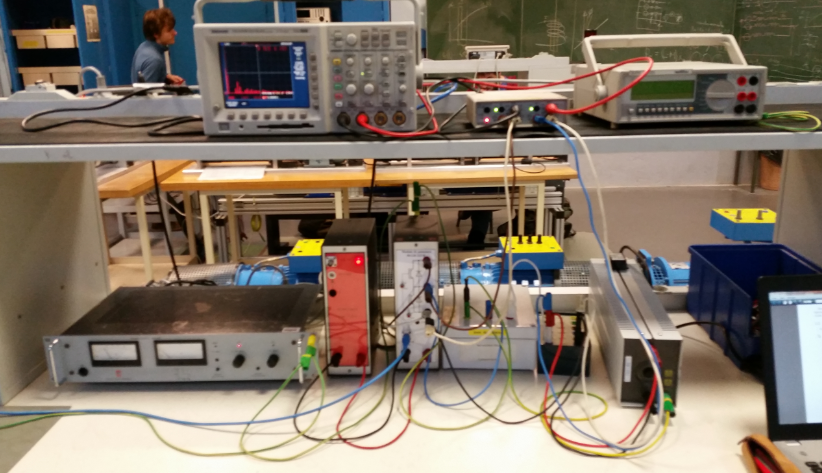
\includegraphics[scale=0.5]{intro1.png}\\
	Premier montage
	\bigbreak
	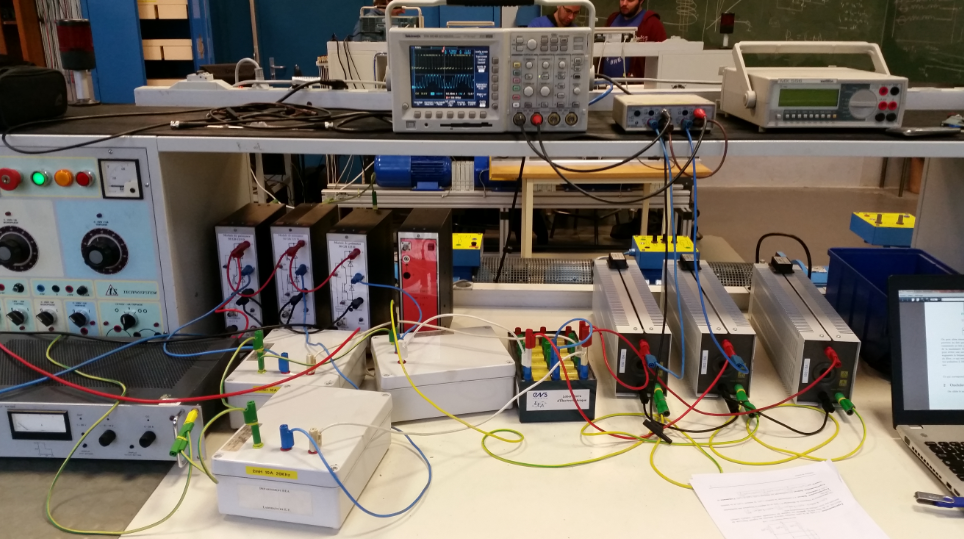
\includegraphics[scale=0.428]{intro2.png}\\
	Deuxième montage
	\end{center}

	\newpage
	
	\section{Cellule de commutation : bras d'onduleur}
	
	On considère les temps de commutation des transistors nuls, les temps de retard de la commande nuls. On définit le signal de commande com(t) de sorte que si :
	\begin{align} &\left \{\begin{matrix}
	 com(t) = 1 & alors& v(t) = U_0\\com(t) = 0 & alors& v(t) = 0
	\end{matrix}\right. &\textbf{donc : 	}&v(t) = com(t).U_0
	\end{align}

Pour réaliser le signal com(t), on compare une modulante m(t) avec une porteuse p(t).Com(t)=1 si la porteuse est supérieur à la modulante : 

\begin{center}
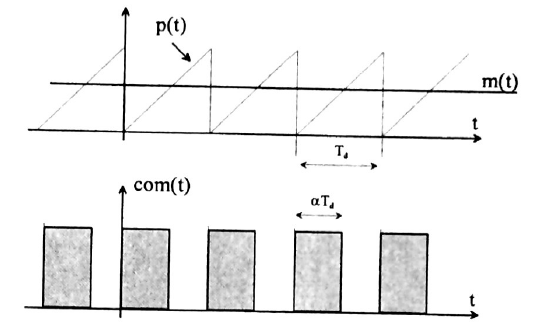
\includegraphics[scale=0.3]{enonce1.png}
\end{center}
	
La porteuse a une période notée $T_d$ dans laquelle elle varie linéairement entre 0 et 1 et la modulante prend aussi ses valeurs dans le même intervalle.\\
On a donc pour $t \in [0;T_d]$ , $p(t) = \frac{t}{T_d}$\\

On fait l'hypothèse que la modulante est constante sur une durée égale à la période de découpage, c'est à dire que pour $t \in [kT_d;(k+1)T_d]$ , $ \forall k \in \mathbb{N}$, $m(t) = m(kT_d)$\\
On pose $\alpha \in [0;1]$ de sorte que $t = kT_d + \alpha T_d$ et $t' \in [0;T_d]$ tel que $t' = t-kT_d$.\\
$\alpha$ étant alors choisi de sorte que :
\begin{align*}
p(t') &= m(t)\\
\text{ie,	} p(\alpha T_d) &= m(kT_d)\\
\text{donc,	} \alpha \frac{T_d}{T_d} &= m(kT_d)
\end{align*}
		Et ceci pour tout $k \in \mathbb{N}$. On constate que alpha est donc aussi fonction continue de variation lente par rapport à $T_d$ et que $\alpha(t) = m(t)$.\\
		\bigbreak
		\bigbreak
		On impose la modulante $m(t) = \frac{1}{2} + \frac{x(t}{2}$ avec $x(t) = \hat{X}sin(\omega t)$ et $\frac{2\pi}{T_d}=10\omega$. On observe les courbes p(t), m(t) et com(t) sur les graphes ci-dessous. On constate sur le spectre en fréquence de com(t), la présence de la fréquence de la modulante et de la porteuse, ainsi que leurs harmoniques d'ordre supérieur.\\
		
		\begin{center}
		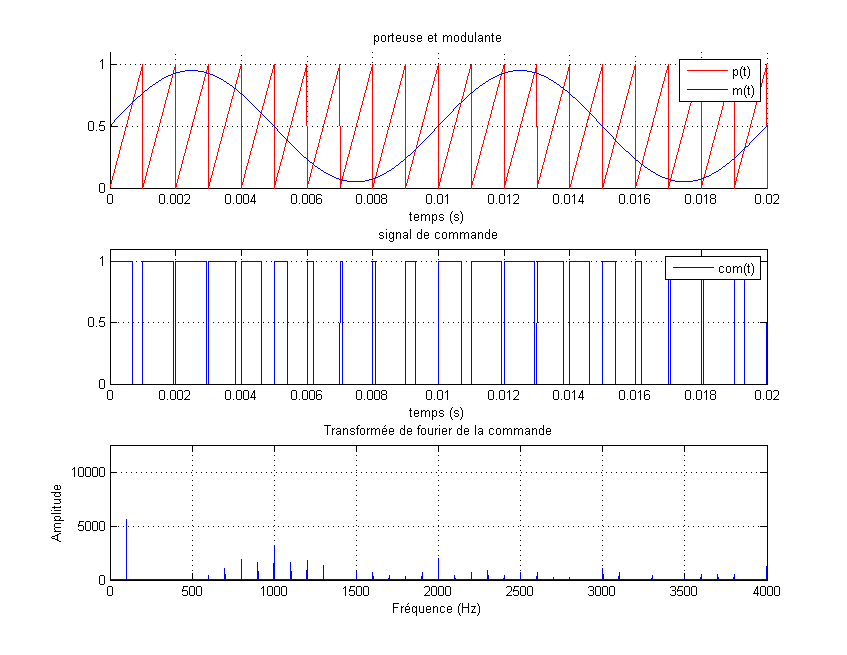
\includegraphics[scale=0.5]{courbe1.png}
		\end{center}
\subsection{Génération du signal de commande}
A l'aide de la carte DSPACE associé au logiciel SIMULINK de Matlab et du bloc PWM, on génère le signal com(t), le bloc PWM génère lui même la porteuse et effectue la comparaison avec la modulante. Il n'est donc nécessaire que de générer celle-ci :

\begin{center}
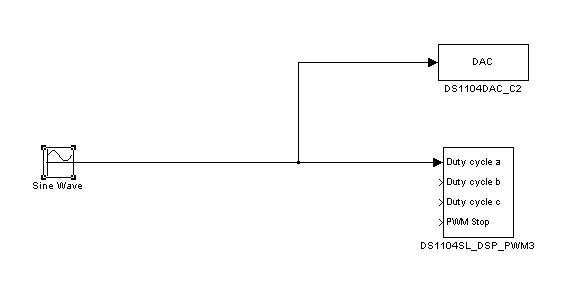
\includegraphics[scale=0.4]{simulink.png}
\end{center}
	\bigbreak
	
	On observe alors le signal com généré ainsi que l'image de x(t) permettant de créer la modulante à l'oscilloscope et ceci pour plusieurs amplitudes (0.3 puis 0.5):
	\begin{center}
	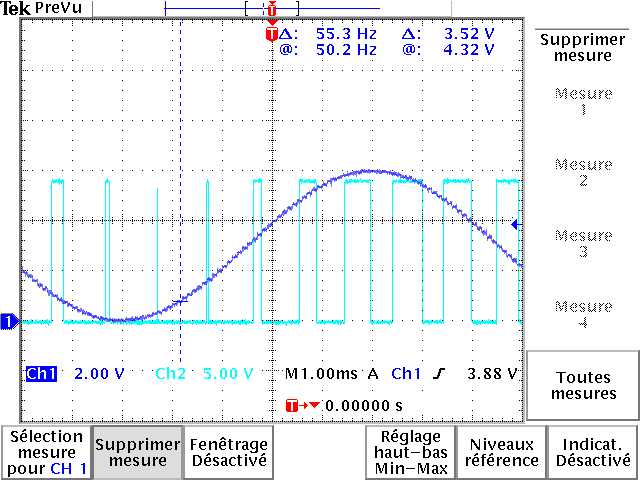
\includegraphics[scale=0.3]{amp03f100.png}
	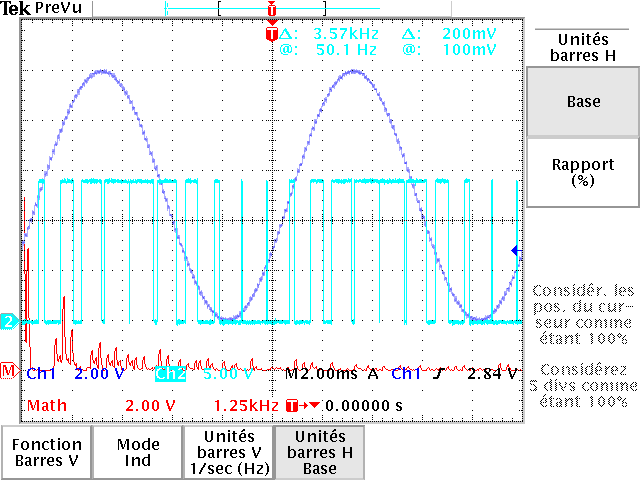
\includegraphics[scale=0.3]{amp05f100.png}
	\end{center}
	On constate que l'on a bien une largeur d'impulsion dépendante de l'amplitude de la modulante. Pour une amplitude proche de 1, les impulsion hautes sont confondu. Pour une amplitude proche de 0, les impulsions basses sont aussi presque confondu.\\
	
	Si l'on s'intéresse au spectre de fréquence du signal de commande :
	\begin{center}
	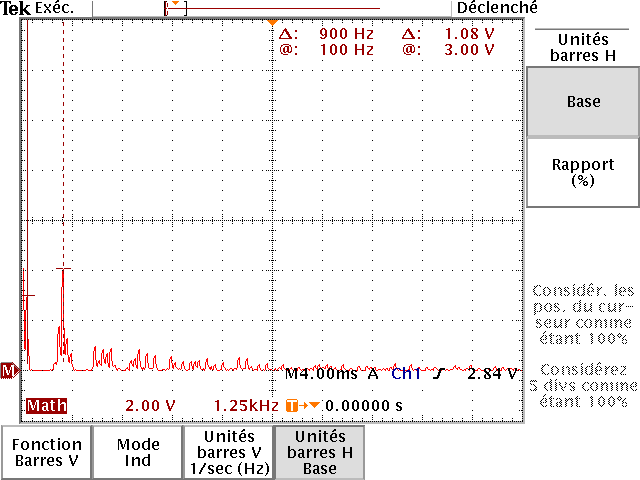
\includegraphics[scale=0.4]{fftm03f100.png}
	\end{center}
	On observe que l'on a bien deux fréquences à 100Hz et 1kHz ainsi que quelques harmoniques d'ordre supérieur. \\
	
	Remarque : Si l'on moyenne le signal de commande, on observe une sinusoïde à la fréquence 100Hz légèrement déphasé, c'est à dire, que le moyenneur agit comme un filtre passe bas. Ceci peut être utile pour vérifier la fréquence d'un tel signal de commande.
	\subsection{Réalisation de l'onduleur monophasé}
	
	On câble l'onduleur monophasé comme sur la figure suivante :
	\begin{center}
	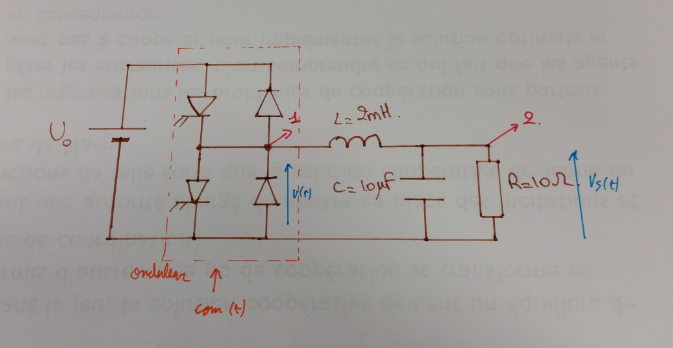
\includegraphics[scale=0.5]{schema1.png}
	\end{center}
	\noindent La fréquence de découpage est toujours de 1kHz.\\
	On relève à l'oscilloscope les tensions v(t) et $v_s$(t):
	\begin{center}
	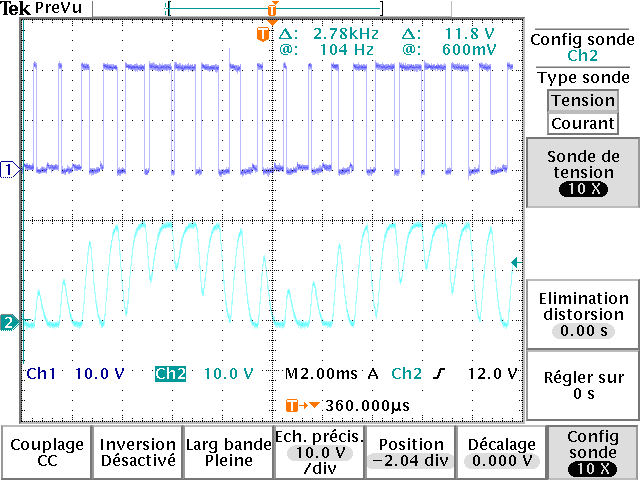
\includegraphics[scale=0.4]{vvs.png}
	\end{center}
	
	Et l'on relève leurs spectres en fréquences à gauche de v et à droite de $v_s$:
	\begin{center}
	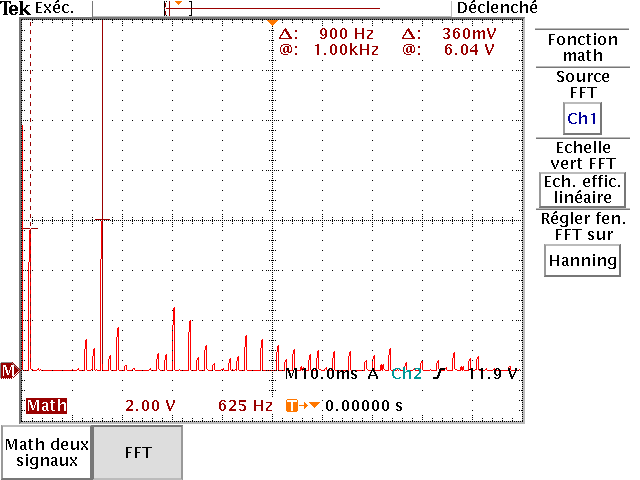
\includegraphics[scale=0.3]{fft_v.png}
	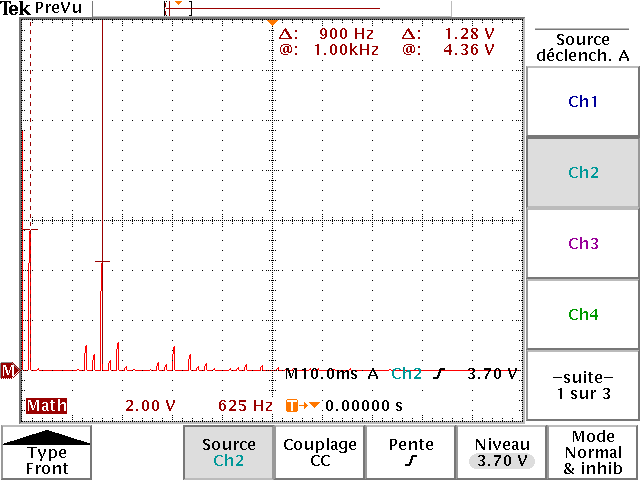
\includegraphics[scale=0.3]{fft_vs.png}
	\end{center}
	On remarque que le filtre RLC (filtre d'ordre 2) a atténué les basses fréquences de $v(t)$, cependant le spectre de $vs(t)$  reste riche en fréquences, car sa fréquence de coupure $f_c=\frac{1}{2\pi\sqrt{LC}}=1.15 k\Omega$ . On effectue alors un essai en réglant la fréquence de la porteuse à 10kHz, et l'on prend une valeur moyenne égale à l'amplitude pour le signal modulant. On observe alors les courbes de $vs(t)$ et sa représentation fréquentielle :
	\begin{center}
	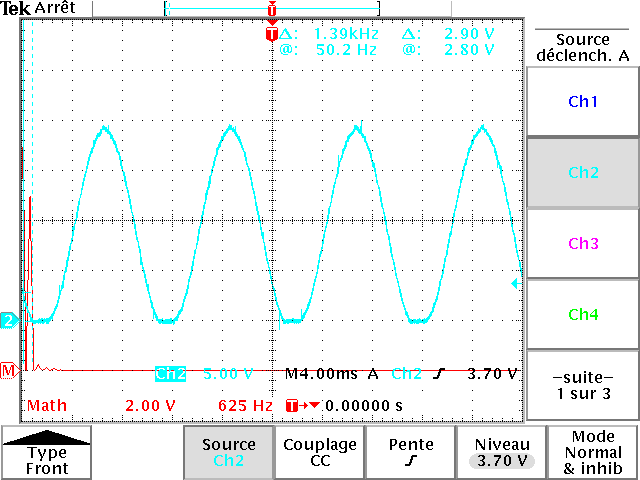
\includegraphics[scale=0.5]{fft_vs_10000.png}
	\end{center}	
	On peut alors remarquer deux chose :\\
	La première est qu'on à une sorte de saturation sur la partie basse, cela provient du fait que l'onduleur nécessite une marge au dessus de 0 (et juste en dessous de 1) que le signal de commande ne doit pas franchir sans entrainer de saturation (haute ou basse). On relève donc la valeur moyenne de la modulante fixée à 0.5 et son amplitude à 0.4 de sorte à avoir 10\% de marge au dessus et au dessous pour éviter une saturation (et donc une partie de l'enrichissement spectral).
	La deuxième est que lorsque l'on augmente la fréquence de découpage à 10kHz, celle-ci est alors  supérieur d'une décade de la fréquence de coupure du filtre, ce qui entraine une atténuation de 40dB environ des hautes fréquences. On observe donc sur le spectre une pulsation à 100Hz (fréquence de la modulante) et une composante continue. Ceci nous permet donc de dire que :
	\[\boxed{v_s = \frac{U_0}{2} + x(t)\frac{U_0}{2}}\]
	Ce qui correspond donc à la composante basse fréquence de la tension v.
	\newpage
	\section{Onduleur triphasé}
	On câble le montage de l'onduleur triphasé suivant avec pour chaque bras d'onduleur et avec $U_0 = 15V$ et on génère trois signaux de commande déphasé de $\frac{2\pi}{3}$ à l'aide de la carte DSPACE.
	\begin{center}
	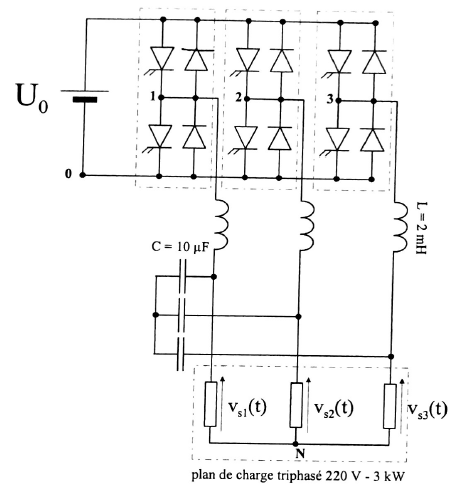
\includegraphics[scale=0.5]{schema2.png}
	\end{center}

Avec une fréquence de découpage de 1kHz, on obtient pour $v_{s1}$ et $v_{s2}$ les deux courbes suivantes :	
	\begin{center}
	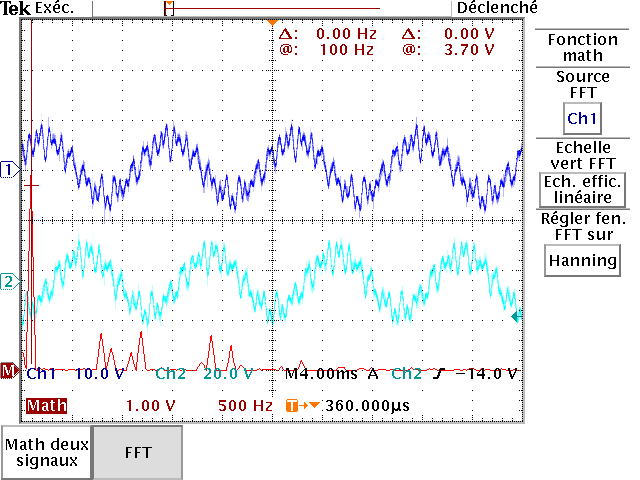
\includegraphics[scale=0.4]{triphase_vs12_1k.png}
	\end{center}
	
	Le filtrage n'étant pas satisfaisant comme expliqué dans la partie précédente. On fixe la fréquence de découpage à 10kHz pour les prochaines manipulations. On ne va observe que deux phases à la fois par limitation du nombre de sondes de courant. Mais chaque phase est effectivement déphasée de $\frac{2\pi}{3}$ par rapport aux autres, et elles se comportent toute de la même façon.\\
	Si l'on remesure $v_{s1}$ et $v_{s2}$ et l'on obtient :
	\begin{center}
	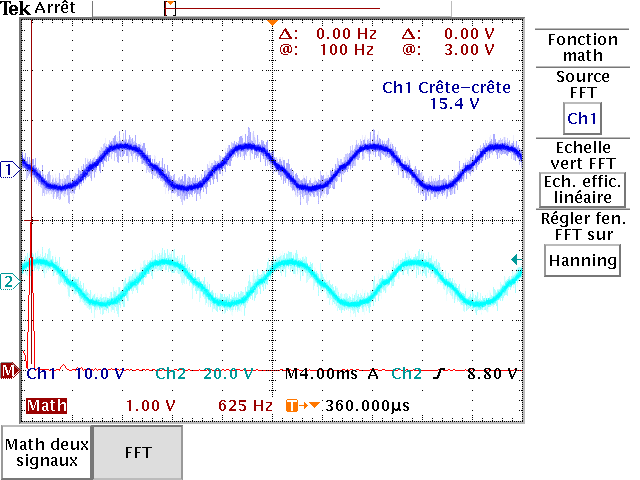
\includegraphics[scale=0.4]{triphase_vs12_10k.png}
	\end{center}
	On observe alors deux sinusoïdes d'amplitude crête à crête de 15V, et sachant que $U_0=15V$, on a:
	\[\begin{matrix}v_{si}(t)=x_i(t)\frac{U_0}{2} &\forall i \in \{1,2,3\}\end{matrix}\]
	On remarque que le spectre est bien débarrassé de la plus part des hautes fréquences.
	\bigbreak
	\bigbreak
	On s'intéresse maintenant à la tension entre le point N et la masse :
	\begin{center}
	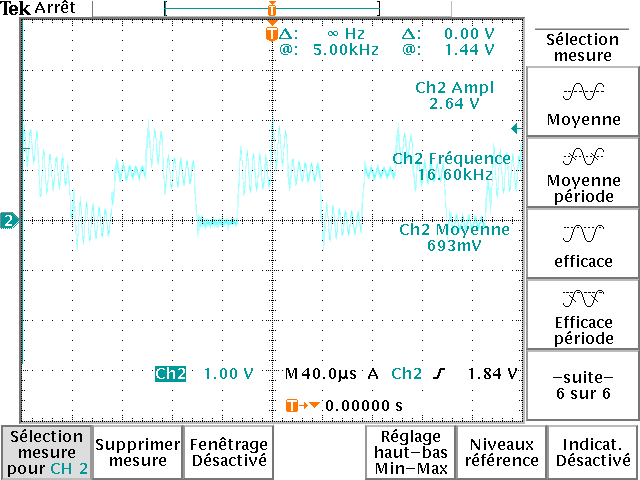
\includegraphics[scale=0.4]{v0n.png}
	\end{center}
	On constate que le point N n'est pas fixe, il oscille à une fréquence de 16.6kHz avec une amplitude crête-crête de 2.6V et une valeur moyenne de 0.7V. On peut considérer qu'il est a peu prés constant.\\
	\bigbreak
	En s'intéressant à la tension entre la borne commune des condensateurs et le neutre :
	\begin{center}
	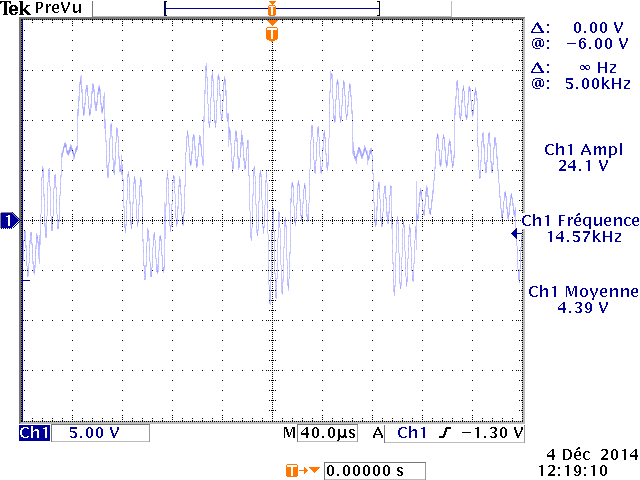
\includegraphics[scale=0.4]{vc0.png}
	\end{center}
	On constate que ce point est aussi flottant, avec une amplitude crête-crête de 24V et une valeur moyenne de 4.4V et une fréquence de 14.6Hz.\\
	On constate donc que l'étude n'est pas aisée et que $v_{1N}$ va aussi beaucoup varier :
\begin{center}
	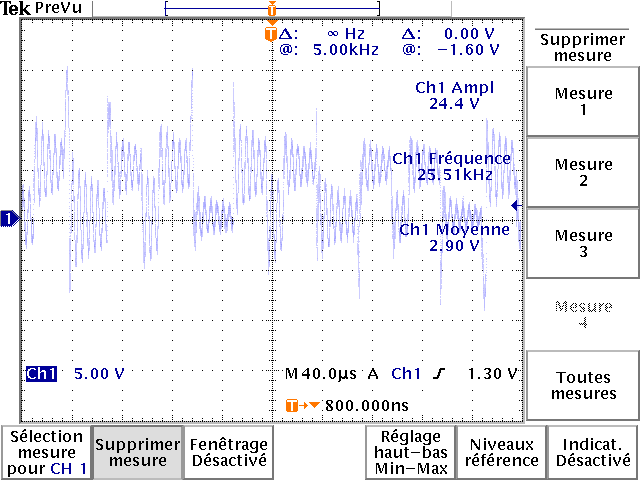
\includegraphics[scale=0.4]{v1n.png}
	\end{center}
	\bigbreak
	\bigbreak
	Si l'on regarde les tensions $v_{10}$ et $v_{20}$ on constate qu'elles sont bien déphasées de $\frac{2\pi}{3}$ de même si on s'intéresse à $v_{30}$ et $v_{20}$ :
	\begin{center}
	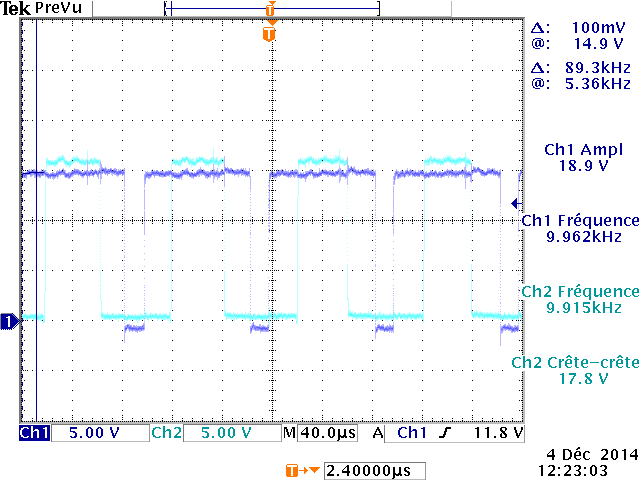
\includegraphics[scale=0.3]{v120.png}
	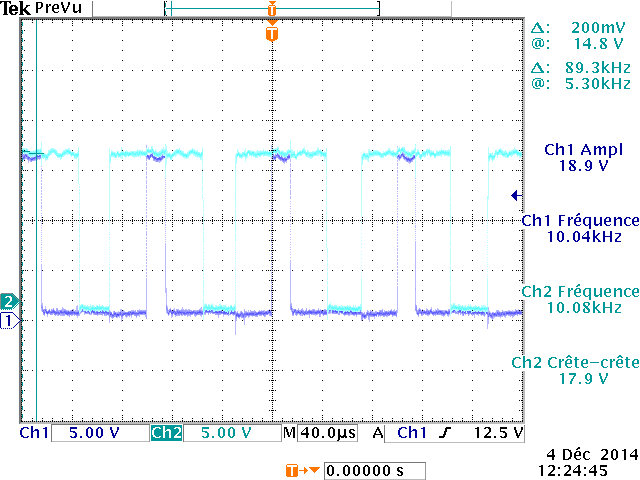
\includegraphics[scale=0.3]{v230.png}
	\end{center}
	On s'attend donc à ce que, avec $a = e^{j\frac{2\pi}{3}}$, pour :
	\[\vec{v(t)} = \sqrt{\frac{2}{3}}(v_1(t)+av_2(t)+a^2v_3(t))\] 
	On devrait avoir,
	\[\vec{v(t)}=\vec{0}\]
	
	\section{Onduleur de tension piloté en courant}
	Nous n'avons malheureusement pas eu le temps de traiter cette partie.
	\section{Conclusion}
	L'étude d'un onduleur monophasé puis d'un onduleur triphasé nous a permis de voir une similitude entre les deux. En effet, on a constaté que l'étude d'un onduleur triphasé revient à étudier trois onduleurs monophasés avec une condition supplémentaire de neutre commun et de condensateur relié. Cependant, l'étude de ce lien n'est pas aisé.\\
	
	De plus, l'utilisation de l'interface DSPACE nous a permis de voir comment générer une tension de commande pour les onduleurs et à quels paramètres il est nécessaire de faire attention(fréquence de découpage, marge haute et basse...).
\end{document}